\documentclass[12pt]{article}
\bibliographystyle{plain}
\usepackage[utf8]{inputenc}
\usepackage{graphicx}
\usepackage{subfigure}
\title
{MSMBuilder 2.5 Tutorial
}

\author{Kyle Beauchamp \and TJ Lane \and Greg Bowman \and  Robert McGibbon \and Vijay Pande}

\begin{document}

\maketitle

\section{Table of Contents}
\begin{enumerate}
\item Installation
\item MSMBuilder Design and Usage
\item MSMBuilder Tutorial
\item Listing of MSMBuilder Scripts
\item Frequently Asked Questions
\end{enumerate}

\newpage

\section{Installation}

\subsection{Prerequisites}
\begin{itemize}
 \item CPU with SSE3 support.
\item GCC 4.2 or later (with OpenMP support)
\item Python
\item Numpy
\item Scipy
\item PyTables
\item numexpr
\item fastcluster (for hierarchical clustering)
\item matplotlib (optional for plotting)
\item ipython (optional for interactive mode)
\item pymol (optional for visualization)
\end{itemize}
Note that the Enthought Python Distribution contains most of these prerequisites and provides an easy way to facilitate installation.

\subsection{Install Python and Python Packages}

Rather than individually install the many python dependencies, we recommend that you download the Python2.7 version of the Enthought Python Distribution, which contains almost all (except fastcluster) python dependencies required to run MSMBuilder.  Please use the 64 bit versions, as this will give higher performance in our RMSD code.

Note for OSX users: Enthought represents the easiest way to obtain a working Python installation.  The OSX system Python install is broken and cannot properly build Python extensions, which are required for MSMBuilder installation.

Note: please use a 64 bit version of python (and thus of MSMBuilder).  On certain systems (OSX Lion), 32 bit builds have experienced crashes in the RMSD / Clustering code.

\subsection{Download and Install MSMBuilder}

Download MSMBuilder, unzip, move to the msmbuilder directory.  Install using setup.py:
\begin{verbatim}
python setup.py build
python setup.py install
\end{verbatim}

You may need root privileges during the install step; alternatively, you can specify an alternative install path via --prefix=XXX.  If you performed the install step with “--prefix=XXX”, you need to ensure that

1.  XXX/bin is included in your PATH
2.  XXX/lib/python2.7/site-packages/ is included in your PYTHONPATH

Step (1) ensures that your can run MSMBuilder scripts without specifying their location.  Step (2) ensures that your Python can locate the MSMBuilder libraries.  

\newpage

\section{MSMBuilder Design and Usage}

MSMBuilder has been designed to provide both ease of use and versatility.  To facilitate the workflows of both novices and experts, we have designed MSMBuilder with two modes of operations:

\begin{enumerate}
\item MSMBuilder is a set of python scripts.  
\item MSMBuilder is a library.
\end{enumerate}

Python scripts allow most users to work without writing a single line of Python code.  Advanced users can write their own Python scripts using the MSMBuilder library.  Using MSMBuilder as a library is further described in the MSMBuilder Library Guide; we recommend that users first master the script interface before jumping into the library.  

\newpage

\section{Tutorial}
\subsection{MSM Construction}

\subsubsection{Overview of MSM Construction}
Constructing a Markov State model involves several steps, which are summarized below:
\begin{enumerate}
 \item Simulate the system of interest.
 \item Convert trajectory data to MSMBuilder format.
 \item Cluster and assign your data to determine microstates.
 \item Construct a microstate MSM
 \item Validate microstate MSM
 \item Calculate macrostates using PCCA+
 \item Calculate a macrostate rate matrix using SCRE
 \item Validate the resulting model.
\end{enumerate}

\subsection{Alanine Dipeptide Tutorial}

This section walks users through a complete Markov state model analysis of the Alanine Dipeptide data provided in MSMBuilder.

In the following, we assume that you have properly installed MSMBuilder.  We also assume that you unzipped the MSMBuilder source file into directory ~/msmbuilder/.  If you unzipped the file elsewhere, you will need to change the paths accordingly.  

Finally, in this tutorial we assume that you have installed pymol for viewing conformations.

\subsubsection{Move to tutorial directory, prepare trajectories}
\begin{verbatim}
cd $PREFIX/share/msmbuilder_tutorial 
tar -xvf XTC.tar
\end{verbatim}

Here, $PREFIX$ is the base directory of your msmbuilder installation.

\subsubsection{Create an MSMBuilder Project}
\begin{verbatim}
ConvertDataToHDF.py  -s native.pdb -i XTC
\end{verbatim}

\subsubsection{Cluster your data using Ward's algorithm and the RMSD metric}
WARNING: this step requires a minimum of 3.0 GB of memory for storing a matrix of pairwise RMSD.
\begin{verbatim}
Cluster.py rmsd hierarchical
\end{verbatim}

\subsubsection{Assign data to states}

\begin{verbatim}
AssignHierarchical.py -H Data/Zmatrix.h5 -n 100
\end{verbatim}

\subsubsection{Validate microstate model with relaxation timescales.}
We calculate the relaxation timescales for a sequence of lagtimes $\{1, 2, ..., 25\}$:
\begin{verbatim}
CalculateImpliedTimescales.py -l 1,25 -i 1 -o Data/ImpliedTimescales.dat
\end{verbatim}

Next, we use python to plot the results, specifying the lagtime between frames (1 ps):  

\begin{verbatim}
PlotImpliedTimescales.py -d 1. -i Data/ImpliedTimescales.dat
\end{verbatim}

\begin{center}
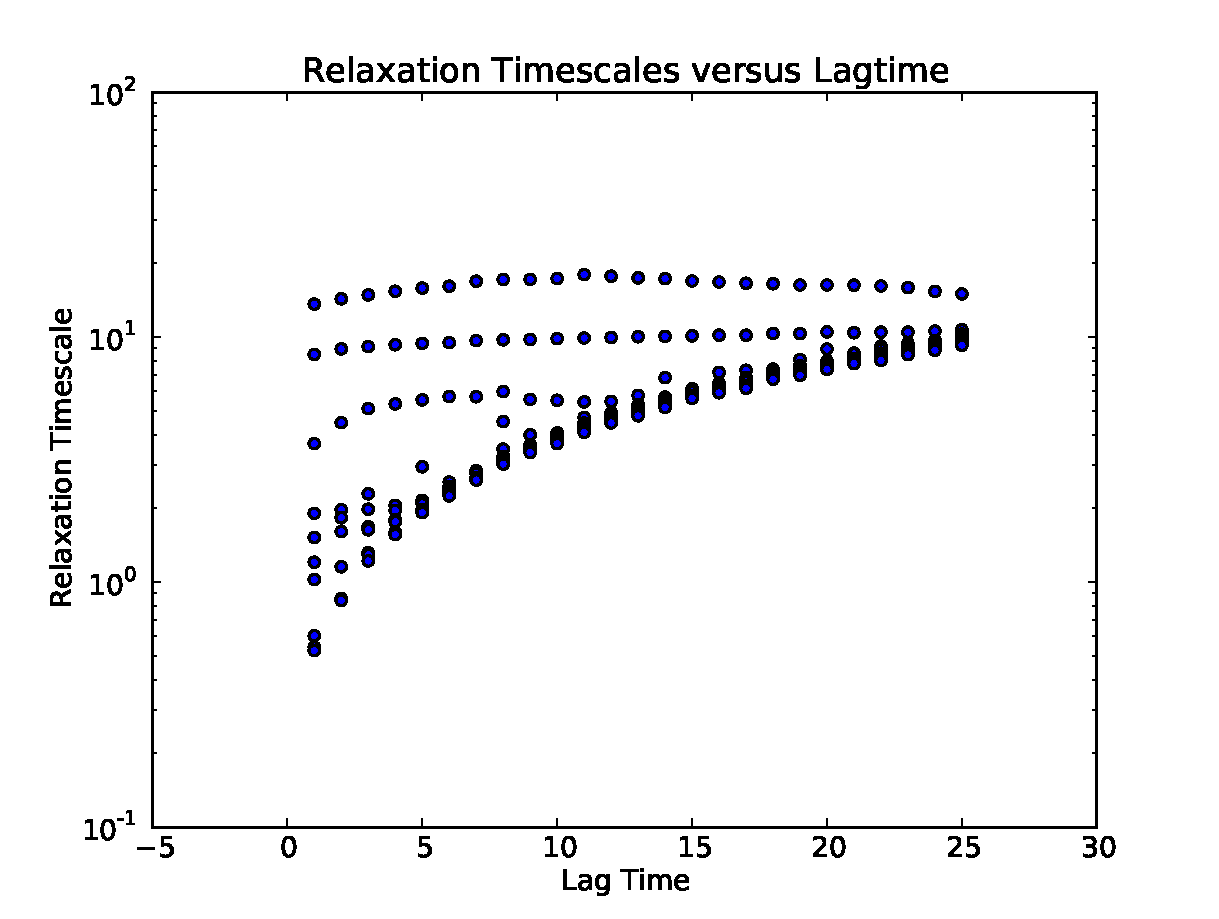
\includegraphics[width=11.7cm]{figures/microstate_timescales.pdf}
\end{center}

\subsubsection{Construct MSM at appropriate lagtime}
The plotted relaxation timescales suggest that the three slow timescales are reasonable flat at a lagtime of 3 timesteps [ps].  Thus, we construct an MSM using that lagtime:

\begin{verbatim}
BuildMSM.py -l 3 
\end{verbatim}

At this point, MSMBuilder has written the following files into your ./Data/ directory:
\begin{verbatim}
Assignments.Fixed.h5
tCounts.UnSym.mtx
tCounts.mtx
tProb.mtx
Mapping.dat
Populations.dat
\end{verbatim}

Assignments.Fixed.h5 contains a “fixed” version of your microstate assignments that has removed all data that is trimmed the maximal ergodic subgraph of your data.  

tCounts.UnSym.mtx contains the raw counts of the ergodic data.  These counts may not be reversible (thus, the count matrix may not be symmetric).  

tCounts.mtx contains the maximum likelihood estimated reversible count matrix.  This is a symmetric matrix.  

tProb.mtx contains the maximum likelihood estimated transition probability matrix.  

Mapping.dat contains a mapping of the original microstate numbering to the “fixed” microstate numbering.  This is necessary because some states may have been discarded during the ergodic trimming step.  

Populations.dat contains the maximum likelihood estimated reversible equilibrium populations.  

\subsubsection{Construct a Macrostate MSM}

Spectral cluster methods such as PCCA+  \cite{Deuflhard2000, Deuflhard2005, kube2007coarse} can be used to construct metastable models with a minimal number of states.  First, we need to construct a microstate model with a short lagtime.  The short lagtime is necessary because PCCA+ tries to create macrostates that are long-lived, or metastable.  At long lagtimes, states become less and less metastable.

\begin{verbatim}
 BuildMSM.py -l 1 -o L1
\end{verbatim}

Our previous examination of the relaxation timescales suggested that there were 3 slow processes, so we choose to build a model with 4 macroscopic states.  

\begin{verbatim}
PCCA.py -n 4 -a L1/Assignments.Fixed.h5 -t L1/tProb.mtx -o Macro4/ -A PCCA+
\end{verbatim}

\subsubsection{Examining the macrostate decomposition}

It is known that the relevant degrees of freedom for alanine dipeptide are the phi and psi backbone angles.  Thus, it is useful to examine (phi,psi), which we have pre-calculated for you.

\begin{verbatim}
./PlotDihedrals.py Macro4/MacroAssignments.h5
\end{verbatim}

You should see the following graph:
\begin{center}
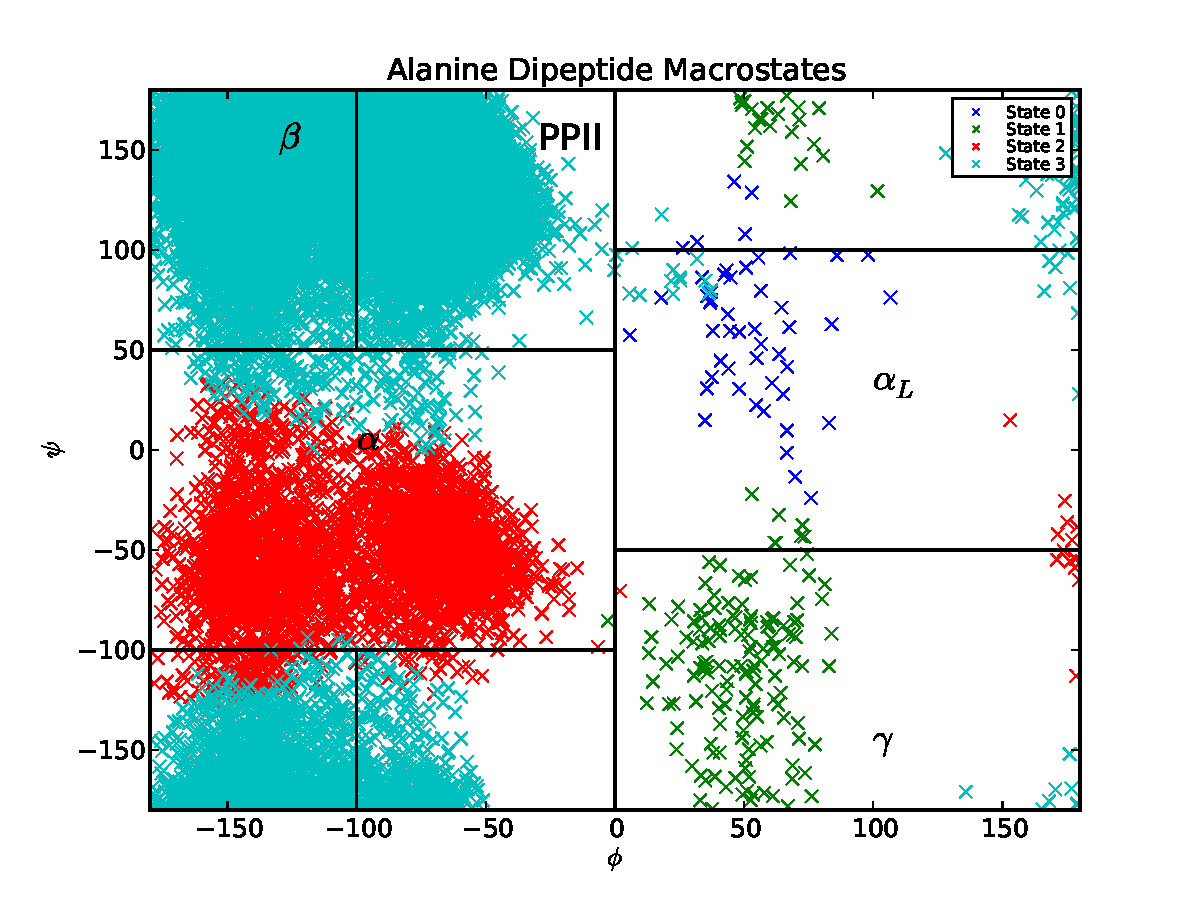
\includegraphics[width=11.7cm]{figures/Macro4}
\end{center}


Thus, the PCCA algorithm has automatically identified the key basins of alanine dipeptide.  The black lines correspond to the $\beta, PP_{II}, \alpha_R, \alpha_L$ and $\gamma$ conformational basins, as estimated previously \cite{Jha2005}.  If we want a model that is less coarse grained, we can build a macrostate MSM with more states.  If, for example, we had used 5 states, we would produce a Ramachandran plot that also captures the barrier between the $\beta$ and $PP_{II}$ basins.  

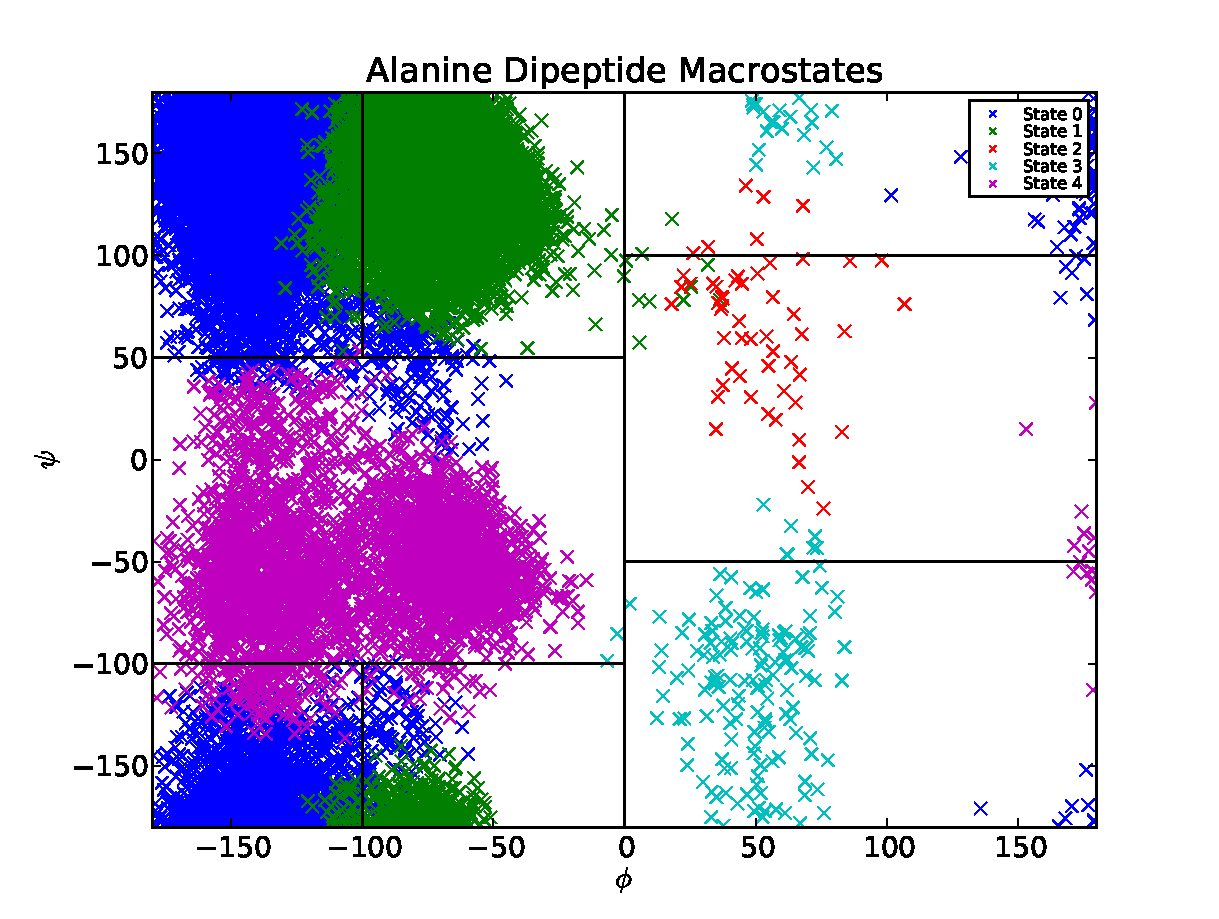
\includegraphics[width=11.7cm]{figures/Macro5}

In general, PCCA and PCCA+ are best applied to capturing long-lived, metastable states.  Thus, for this system, applying PCCA+ to construct models with more than 5 states may not produce useful models.  This is because alanine dipeptide only contains four eigenvalues that are significantly slower than the time resolution of 1 ps.  

\subsubsection{Calculate Macrostate Implied Timescales}

\begin{verbatim}
CalculateImpliedTimescales.py -l 1,25 -i 1 -o Macro4/ImpliedTimescales.dat 
-a Macro4/MacroAssignments.h5 -e 3

PlotImpliedTimescales.py -i Macro4/ImpliedTimescales.dat -d 1
\end{verbatim}

Occasionally, PCCA+ will lead to poor macrostates, so it is important to verify that:

\begin{enumerate}
 \item The state decomposition makes physical sense
 \item The macrostate implied timescales make sense
 \item The macrostate implied timescales ``follow'' the microstate implied timescales
\end{enumerate}

\subsubsection{Estimate a converged rate matrix using SCRE}

In the macrostate implied timescales, the slowest implied timescale converges at approximately 10 ps, while the third timescale converges as 5 ps.  Furthermore, the third timescale is aliased at lagtimes starting with 14 ps; lagtimes longer than 14 ps will not accurately capture the dynamics of this relaxation.  This suggests that this system might benefit from estimating rates using SCRE and multiple lagtimes.  

To build an SCRE model, we first construct a macrostate transition matrix with lagtime 1.  

\begin{verbatim}
 BuildMSM.py -l 1 -a Macro4/MacroAssignments.h5 -o Macro4/
\end{verbatim}

The key idea in SCRE is to estimate rate matrix $K_{ij}(\tau)$ for a variety of lagtimes.  Then, each rate matrix element is fixed when $K_{ij}(\tau)$ becomes approximately constant with respect to the lagtime $\tau$.  The final rate matrix provides estimates of Markovian rates for each of the rate elements $K_{ij}$.  

Next, we run an interactive script to estimate rates using SCRE.  

\begin{verbatim}
 Interactive-SCRE.py -a Macro4/Assignments.Fixed.h5 -o Macro4
\end{verbatim}

In practice, the script will prompt the user to select a maximum lagtime.  The script then estimates and plots rate matrices for each lagtime up to the maximum value.  The user is then asked to identify converged rate matrix elements.  In general, one should try to estimate the quickly-convergign rates first.  After those rates are constrained, one can then try to estimate the slower and / or less Markovian rates.  For concreteness, I used the following inputs:

25
1,0,6
25
3,2,19
25
3,1,6
25
3,0,9
25
14

Note that on the last iteration, the user is asked only to select a lagtime.  

Finally, we compare the fixed-lagtime and SCRE estimates of implied timescales:

\begin{verbatim}
 ./PlotMacrostateImpliedTimescales.py
\end{verbatim}


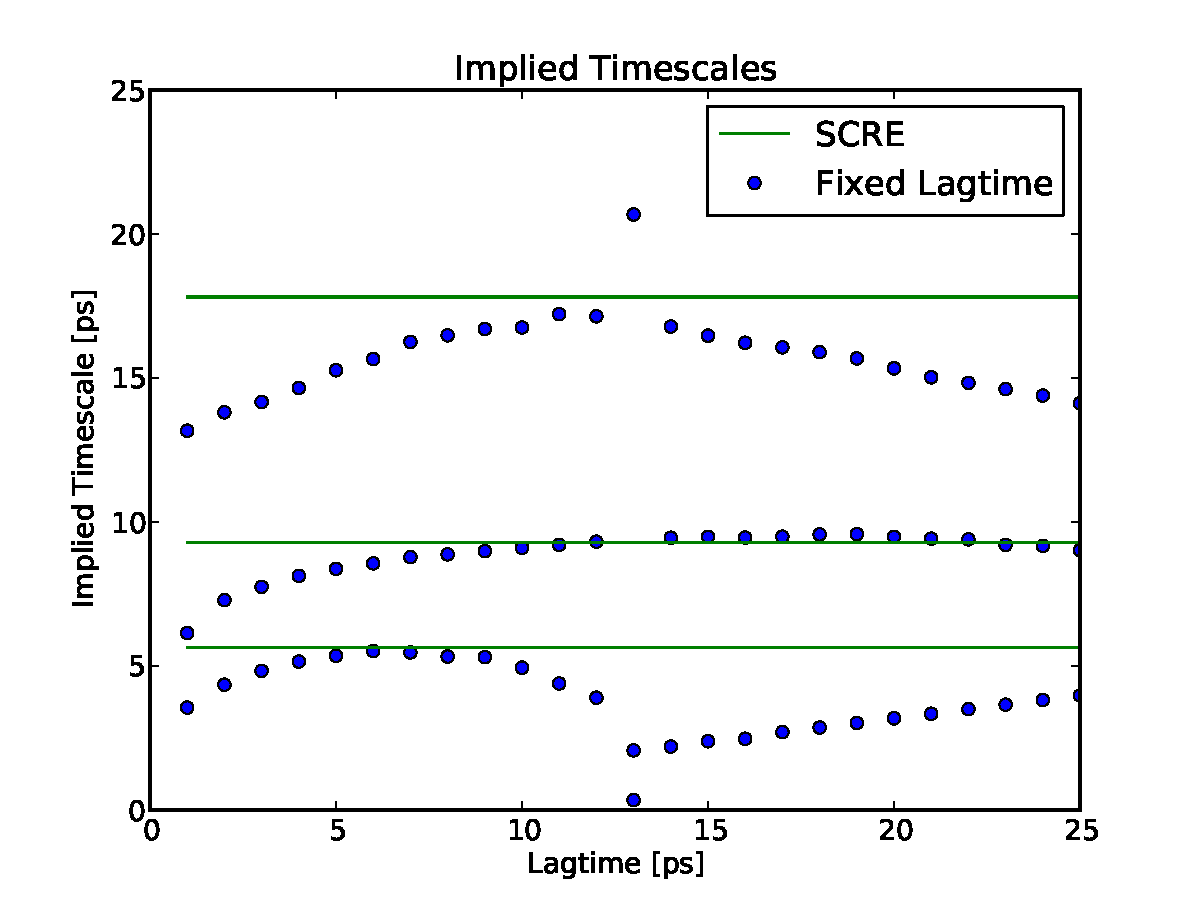
\includegraphics[width=11.7cm]{figures/SCRE}


We find that the SCRE estimates capture the ``converged'' values of the fixed-lagtime timescales.  Achieving convergence for each timescale is not possible with a fixed-lagtime MSM, because the 20 ps lagtime required for the second relaxation causes the third relaxation to alias.  

\newpage

\subsection{MSMBuilder Scripts}

The MSMBuilder scripts are listed below.  Each script below provides instructions by running with the -h flag.  Note that the installer (setup.py) should have installed each script below to someplace in your PATH.  

\subsubsection{ConvertDataToHDF.py}

Merges sequences of XTC or DCD files into HDF5 files that MSMB2 can read quickly.  Takes data from a directory of trajectory directories or a FAH-style filesystem.  

Note: if you wish to convert a pre-existing MSMBuilder1 project, use UpdateProjectToHDF5.py 

\subsubsection{CreateAtomIndices.py}
Selects atom indices you care about and dumps them into a flat text file. Can select all non-symmetric atoms, all heavy atoms, all alpha carbons, or all atoms.

\subsubsection{Cluster.py}

Cluster your data using your choice of clustering algorithm and distance metric.  We have previously used several clustering protocols, which are summarized:

\begin{enumerate}
 \item RMSD + k-centers clustering \cite{Bowman2009c, Bowman2009a} ( ``Cluster.py  rmsd kcenters'')
 \item RMSD + hybrid k-centers / k-medoids clustering \cite{msmb2} (``Cluster.py  rmsd hybrid'')
 \item RMSD + Ward clustering (``Cluster.py  rmsd hierarchical'')
\end{enumerate}

We recommend Ward clustering if it is computationally feasible; otherwise, use the hybrid k-centers / k-medoids clustering.  Ward clustering calculations an $O(N^2)$ distance matrix, which may be prohibitive for datasets with many conformations.  

Most of our experience has been in applying MSMBuilder to protein folding.  Thus, non-folding applications may require a slightly different protocol.

\subsubsection{Assign.py / AssignHierarchical.py}
Assign.py assigns data to the cluster generators calculated using the k-centers or hybrid algorithms.

AssignHierarchical.py assigns data using the output of a hierarchical clustering algorithm such as Ward.  The key difference is that a single hierarchical clustering allows construction of models with any number of states.

\subsubsection{CalculateImpliedTimescales.py}
Calculates the implied timescales for a python range of MSM lag times.  This allows you to validate whether a given model is Markovian.  
	Notes:
\begin{enumerate}
 \item You might get a SparseEfficiencyWarning for every lag time. Ignore this.
 \item Lagtimes are input in units of the time spacing between successive trajectory frames.  If your trajectories are stored every 10 ns, then -l 1,4 estimtes implied timescales with lagtimes 10, 20, 30, 40 ns.  
\end{enumerate}

\subsubsection{PlotImpliedTimescales.py}
A template for generating an implied timescales plot.

\subsubsection{BuildMSM.py}
Estimate a reversible transition and count matrix using a two step process:
\begin{enumerate}
 \item Use Tarjan algorithm to find the maximal strongly-connected (ergodic) subgraph
 \item Use likelihood maximization to estimate a reversible count matrix consistent with your data
\end{enumerate}

This script also outputs the equilibrium populations of the resulting model, as well as a mapping from the original states to the final (ergodic) states.

\subsubsection{GetRandomConfs.py}
Selects random conformations from each state of your MSM. This is very useful for efficient calculation of observables.

\subsubsection{CalculateClusterRadii.py}
Calculates the mean RMSD of all assigned snapshots to their cluster generator for each cluster. Gives an indication of how structurally diverse clusters are.

\subsubsection{CalculateRMSD.py}
Calculate the RMSD between a PDB and a trajectory (or set of cluster centers). Useful for deciding which clusters belong to the folded, unfolded, or transition state ensembles (or any other grouping!)

\subsubsection{CalculateProjectRMSD.py}
Calculates the RMSD of all conformations in a project to a given conformation.

\subsubsection{DoTPT.py}
Performs Transition Path Theory (TPT) calculations. You will need to define good starting (reactants/U) and ending (products/F) ensembles for this script. Writes the forward and backward committors and the net flux matrix

\subsubsection{SavePDBs.py}
Allows you to sample random PDBs from particular states and save them to disk.

\subsubsection{PCCA.py}
Lumps microstates into macrostates using PCCA \cite{Deuflhard2000} or PCCA+ \cite{Deuflhard2005, kube2007coarse}. This script generates a macrostate assignments file from a microstate model.  

Notes:
\begin{enumerate}
 \item We recommend PCCA+ for most applications
 \item PCCA+ requires a reversible MSM as input
 \item You can discard eigenvectors based on their equilibrium flux (fPCCA+).
\end{enumerate}

\newpage

\section{Frequently Asked Questions}

Q1.  How do I decrease / increase the number of threads used during clustering, assignment, and rmsd calculation?

A1.  Set the \begin{verbatim}OMP_NUM_THREADS\end{verbatim} environment variable to the desired number of threads.  In linux, you would type (or add to your bashrc):
\begin{verbatim}
export OMP_NUM_THREADS=6 
\end{verbatim}

\vspace{5mm}

Q2:  I see the following error.  What do I do?
\begin{verbatim}
 #004: H5Z.c line 1095 in H5Z_pipeline(): required filter is not registered
\end{verbatim}

A2:  You are trying to read an HDF5 file that was written using a different PyTables installation.  Your current PyTables installation is likely missing the compression algorithm (filter) required to read the file.  The solution is to find a version of Pytables that has the old compression algorithm (filter) and use MSMBuilder to read and then re-write the trajectories (by default, MSMBuilder uses the PyTables BLOSC compression).  To do this (for a single File), you would so something like:
from msmbuilder import Trajectory
R1=Trajectory.Trajectory.LoadFromLHDF(Filename)
R1.SaveToLHDF(NewFilename)

\vspace{5mm}

Q3: I received an “Illegal instruction” error.  What does this mean?

A3:  MSMBuilder2 requires an SSE3 compatible processor when Clustering and calculating RMSDs.  Any processor built after ~2006 should have the necessary instructions.  

\vspace{5mm}

Q4:  In my implied timescales plot, I see unphysically slow timescales.  

A4:  The current estimators for transition matrices are somewhat sensitive to poor statistics.  The hybrid k-centers / k-kmedoids clustering focuses on providing the best possible clustering--without regard to the quality of the resulting statistics.  Thus, to get more precise timescales, you may have to find a way to achieve better statistics.  Here are a few ideas:
	A.  Collect longer trajectories.
	B.  Use fewer states.  Also, by increasing the number of local and global k-medoid updates, you can often increase the accuracy of your clustering while simultaneously lowering the number of states.  
	C.  Subsample your data when clustering.
	D.  Skip the initial k-centers step of clustering, instead using randomly selected conformations.  This generally leads to poorer clustering quality, but considerably better statistics in each state.  (Thus, the clusters will be much more localized to regions of high population density.)  This can be achieved by setting “-r 0” when clustering.  

\vspace{5mm}

Q5.  Why are there -1s in my Assignments matrix?

A5.  We use -1 as a “padding” element in Assignment matrices. Suppose your project has maximum trajectory length of 100.  If trajectory 0 has length 50, then A[0,50:] should be a vector of -1.  Furthermore, when you perform trimming to ensure (strong) ergodicity, futher -1s could be introduced at the start or finish of the trajectory.  Finally, if Ergodic trimming was performed with count matrices estimated using a sliding window, you could even see something like:
-1 -1 -1 x -1 -1 y z …
This is because sliding window essentially splits your trajectory into independent subtrajectories--one for each possible window starting position.  “x” then marks the start of one of these subtrajectories.

\bibliography{Tutorial}


\end{document}